\documentclass[a4paper, 12pt]{article}

% a nice font
\usepackage{kpfonts}

% basic text stuff
\usepackage[utf8]{inputenc}
\usepackage[T1]{fontenc}

\usepackage{tikz} % main tikz package
\usepackage{tikz-network} % for network / graph utilities

% for a nicer colorscheme
\definecolor{blue}{rgb}{0.38, 0.51, 0.71} %glaucous, 97,130,181, #6182B5
\definecolor{darkblue}{RGB}{17, 42, 60} % 112A3C
\definecolor{red}{RGB}{175, 49, 39} % AF3127

\definecolor{orange}{RGB}{217, 156, 55} % D99C37
\definecolor{green}{RGB}{144, 169, 84} % 90A954
\definecolor{palegreen}{RGB}{197, 184, 104} % C5B868

\definecolor{yellow}{RGB}{250, 199, 100} % FAC764
\definecolor{brokenwhite}{RGB}{218, 192, 166} % DAC0A6
\definecolor{brokengrey}{rgb}{0.77, 0.76, 0.82} % {196,194,209}, C4C2D1


\begin{document}
    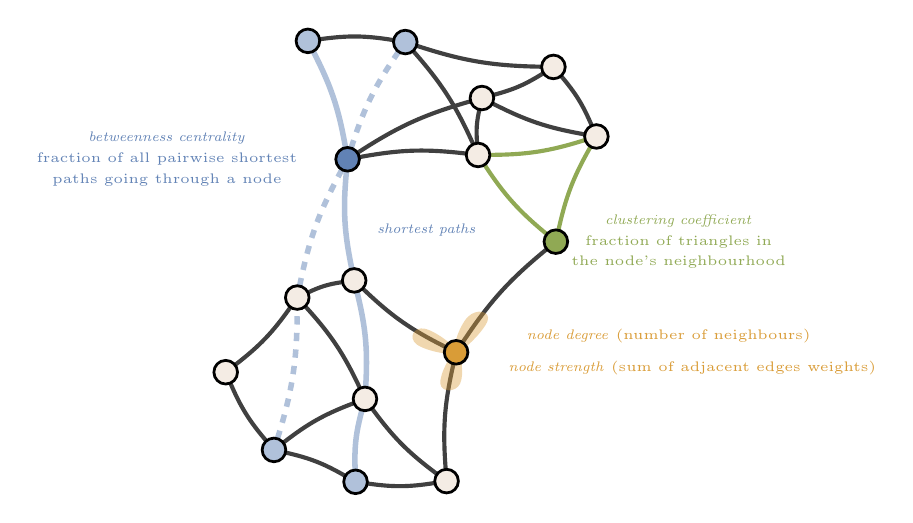
\begin{tikzpicture}[>=stealth']
        %\clip (0,0) rectangle (6,6);
        \coordinate (13) at (3.572,1.845);
        \fill [orange, opacity=0.4] plot [smooth cycle, tension=1] coordinates {(13) ($ (13) + (-0.4,0.3)$) ($ (13) + (-0.5,0.1)$)};
        \fill [orange, opacity=0.4] plot [smooth cycle, tension=1] coordinates {(13) ($ (13) + (-0.2,-0.4)$) ($ (13) + (0.05,-0.4)$)};
        \fill [orange, opacity=0.4] plot [smooth cycle, tension=1] coordinates {(13) ($ (13) + (0.15,0.45)$) ($ (13) + (0.4,0.4)$)};

        \node (degree) at ($ (13) + (2.7,0.2) $)
        {\color{orange}{\tiny{\emph{node degree} (number
        of neighbours)}}};
        \node (degree) at ($ (13) + (3,-0.2) $)
        {\color{orange}{\tiny{\emph{node strength} (sum of adjacent edges
        weights)}}};

        \Vertex[color=brokenwhite!30,x=3.9,y=5.074,size=0.3,]{0}
        \Vertex[color=brokenwhite!30,x=3.851,y=4.351,size=0.3,]{1}
        \Vertex[color=brokenwhite!30,x=5.354,y=4.586,size=0.3,]{2}
        \Vertex[color=green, x=4.839,y=3.250,size=0.3,]{3}
        \node (clustering) at (6.4,3.25) {\color{green}{\tiny{\shortstack{\emph{clustering coefficient}\\ fraction of triangles in \\ the node's neighbourhood}}}};
        \Vertex[color=blue!50, x=2.927,y=5.785,size=0.3, ]{4}
        \Vertex[x=1.690,y=5.800,size=0.3,color = blue!50, ]{5}
        \node (shortest) at (3.2,3.4) {\color{blue}{\tiny{\emph{shortest paths}}}};
        \Vertex[x=2.194,y=4.296,size=0.3,color = blue]{6}
        \node (centrality) at (-0.1, 4.3)
        {\color{blue}{\tiny{\shortstack{\emph{betweenness centrality}\\
        fraction of all pairwise shortest \\ paths going through a node}}}};
        \Vertex[color=brokenwhite!30,x=4.808,y=5.469,size=0.3,]{7}
        \Vertex[color=brokenwhite!30,x=0.646,y=1.592,size=0.3,]{8}
        \Vertex[color=brokenwhite!30,x=2.415,y=1.253,size=0.3,]{9}
        \Vertex[x=2.295,y=0.200,size=0.3, color = blue!50,]{10}
        \Vertex[color=blue!50,x=1.259,y=0.605,size=0.3,]{11}
        \Vertex[color=brokenwhite!30,x=2.278,y=2.758,size=0.3,]{12}
        \Vertex[color=orange,x=3.572,y=1.845,size=0.3,]{13}
        \Vertex[color=brokenwhite!30,x=1.555,y=2.540,size=0.3,]{14}
        \Vertex[color=brokenwhite!30,x=3.451,y=0.209,size=0.3,]{15}
        \Edge[,bend=-8.531](0)(1)
        \Edge[,bend=-8.531](0)(2)
        %\Edge[,bend=-8.531](0)(5)
        \Edge[,bend=-8.531](0)(6)
        \Edge[,bend=-8.531](0)(7)
        \Edge[color=green,bend=-8.531](1)(2)
        \Edge[color=green,bend=-8.531](1)(3)
        \Edge[,bend=-8.531](1)(4)
        \Edge[,bend=-8.531](1)(6)
        \Edge[color=green,bend=-8.531](2)(3)
        \Edge[,bend=-8.531](2)(7)
        \Edge[,bend=-8.531](3)(13)
        \Edge[,bend=-8.531](4)(5)
        \Edge[lw=2, color=blue!50 ,bend=8.531](5)(6)
        \Edge[,bend=-8.531](4)(7)
        \Edge[lw=2, color=blue!50, style={dashed},bend=-8.531](4)(6)
        \Edge[lw=2, color=blue!50 ,bend=-8.531](6)(12)
        \Edge[lw=2, color=blue!50, style={dashed},bend=-8.531](6)(14)
        %\Edge[,bend=-8.531](8)(10)
        \Edge[,bend=-8.531](8)(11)
        %\Edge[,bend=-8.531](8)(12)
        \Edge[,bend=-8.531](8)(14)
        \Edge[lw=2, color=blue!50,bend=-8.531](9)(10)
        \Edge[lw=2, color=blue!50 ,bend=-8.531](9)(12)
        \Edge[,bend=-8.531](9)(14)
        \Edge[,bend=-8.531](9)(15)
        \Edge[,bend=-8.531](10)(11)
        \Edge[,bend=-8.531](9)(11)
        \Edge[lw=2, color=blue!50, style={dashed},bend=-8.531](11)(14)
        \Edge[,bend=-8.531](10)(15)
        \Edge[,bend=-8.531](12)(13)
        \Edge[,bend=-8.531](12)(14)
        %\Edge[,bend=-8.531](13)(14)
        \Edge[,bend=-8.531](13)(15)
   \end{tikzpicture}
\end{document}
